\documentclass[handout]{BeamerTemplate}

\title{Module 2 - Variables aléatoires à une dimension}

\date{\today}

\begin{document}
\begin{frame}[t]
  \titlepage
\end{frame}

%-------------------------------------------------------------------------------------------------------------------------------------





%%%%%%%%%%%%%%%%%%%%%%%%%%%%%%%%%%%
%%%%%%%%%%%%%%%%%%%%%%%%%%%%%%%%%%%
%%%%%%%%%%%%%%%%%%%%%%%%%%%%%%%%%%%


\section[Intro]{Introduction}
\subsection*{ }

%\subsection{Définitions et notation}

\begin{frame}[t]{Exemple 1}
Le résultat d'une expérience aléatoire est souvent un nombre réel, ou encore on assigne une valeur réelle aux résultats possibles d'une expérience.

\medskip
{\ }

\uncover<2->{
% {\bf \underline{Exemple 1}:}\\
 ${\cal E}$: On tire une pièce de monnaie 2 fois
 %et on associe une valeur  réelle $x$ à chaque élément de l'espace échantillonnal

 $S=\{FF,FP,PF,PP\}$.

 \medskip
 Exemple de valeur associée à chaque résultat: le nombre de fois où Pile apparaît. On peut noter cette variable $X$.

 \begin{tabular}{ll}
 $X=0$  &si le résultat  est $FF$,\\
 $X=1$ &si le résultat est $FP$ ou $PF$,\\
 $X=2$ &si le résultat est $PP$.
 \end{tabular}
}
\end{frame}

\begin{frame}[t]{Variable aléatoire}
%En fait pour toute expérience aléatoire ${\cal{E}}$ avec espace échantillonnal $S$, rien ne nous empêche de définir une fonction, disons $X$, qui prend en entrée un résultat de l'expérience aléatoire (donc $e\in S$) et qui donne en sortie un nombre réel, $x=X(e)$.

Soit ${\cal{E}}$ une expérience aléatoire ayant
  comme espace échantillonnal $S$.

 \begin{Boite}{Variable aléatoire}
 \begin{itemize}\itemsep3mm
\item  Soit $X: S\to \mathbb{R}_X$, une fonction  qui associe un nombre réel $X(e)$ à chaque élément
  $e\in S$. Alors on appelle $X$ une \alert{variable aléatoire}.

\item  $\mathbb{R}_X$ est l'ensemble des valeurs que peut prendre $X$ et est appelé \alert{image de $X$} ou \alert{support de $X$}.
\end{itemize}
 \end{Boite}

\end{frame}

\begin{frame}[t]{Exemple 2}
${\cal{E}}$: on lance un dé régulier et on observe la face du dessus. \\
$S=\{1,2,3,4,5,6\}$.\\
On peut définir une infinité de variables aléatoires. \\
Voici 2 exemples.

 \begin{itemize}
  \item<2-> $X$ est la variable aléatoire qui donne le  résultat observé.\\
    $X(e)=e,~\forall e\in S$\\
    $\mathbb{R}_X=\{1,2,3,4,5,6\}$
  \item<3-> Je gagne 50\$ si je roule  4, 5 ou 6.\\
    Je perds 75\$ si je roule 1, 2 ou 3.\\
    $Y$ est la variable aléatoire qui représente mon gain.\\
      $Y(e)=\left\{
  \begin{array}{rl}
  -75 &\text{si}\;e\in\{1,2,3\}\\
  50&\text{si}\;e\in\{4,5,6\}
  \end{array}
  \right.$\\
  $\mathbb{R}_Y=\{-75,50\}$.
 \end{itemize}
\end{frame}


\begin{frame}[t]{Exemple 2: probabilités}

Quelle est la probabilité que je perde 75 \$ en jouant?\\

%Puisque les événements $A$ et $B$  sont équivalents, leur probabilité est égale. Si le dé est équilibré, quelle est la probabilité que $Y$ prenne la valeur $-1$?

{\large
 \begin{tabular}{c|c|c|c}\hline
 $e$ & $X(e)$ & $Y(e)$ & $P(e)$ \\ \hline
  1 & & & 1/6 \\
  2 & &  & 1/6  \\
  3 & &  & 1/6  \\
  4 & &  & 1/6  \\
  5 & &  & 1/6  \\
  6 & &  & 1/6  \\ \hline
 \end{tabular}
}


\end{frame}

\begin{frame}[t]{Événements de $S$ et sous-ensembles de $\mathbb{R}_X$}
Pour une variable aléatoire $X: S\to \mathbb{R}_X$, à tout sous-ensemble de $\mathbb{R}_X$ correspond un sous-ensemble de $S$.
On pourra donc appliquer les règles de calculs de probabilités
vues au chapitre 1 aux calculs de probabilités portant
sur la valeur de variables aléatoires.

\bigskip

\uncover<2->
{
Si on prend $Y$ de l'exemple 2, alors $Y\neq-75$ équivaut à l'événement
$A=\{4,5,6\}$, le complément de l'événement $\bar{A}=\{1,2,3\}$. $Y\neq-75$
est donc aussi l'événement $Y=50$. 

Ainsi $P(Y\neq -75)=P(A)=1-P(\bar{A})=1-P(Y=-75)$.
}
\end{frame}

%\begin{frame}[t]{Image inverse}
%On dénote souvent l'ensemble des événements de $S$ qui
%consitituent un événement $B$ dans $R_X$ l'\alert{image
%inverse de $B$}:
%$$ X^{-1}(B)=\{e\in S:X(e)=B\}.$$
%{\it (Généralement, quand on travaille avec une v.a. $X$ on s'intéresse
%plus à $R_X$ qu'à $S$.)}
%
%\uncover<2->{
% Dans l'exemple du dé avec $B=\{-1\}$:
% $$P_Y(B)=P[Y^{-1}(B)]=P(\{e\in S:Y(e)=-1\})=P(\{1,2,3\})=3/6.$$
%}
%\end{frame}
%
%\begin{frame}[t]{Un autre exemple}
%
%{\small
% Un réseau électrique est fonctionnel si au moins 2 des 3 lignes
% de transmission principales ne sont pas surchargées. Si `$S$' dénote
% une ligne surchargée et `$P$' dénote une ligne non surchargée, alors
% on peut représenter l'espace échantillonnal par
% $$S=\{PPP,PPS,PSP,SPP,SPS,SSP,PSS,SSS\}.$$
%
% Soit $X$, la v.a. qui vaut 1 si le réseau fonctionne et 0 sinon. Quelles
% sont les probabilités de chaque valeur possible de $X$ si les trois lignes
% sont indépendantes et si chaque ligne est surchargée avec probabilité
% 0.1?
%}
%\end{frame}
%
%
%\begin{frame}[t]{Exemple (suite)}
%
%{\large
%\begin{center}
% \begin{tabular}{c|c|c}\hline
% $e$ & $X(e)$ & $P(e)$ \\ \hline
%  PPP & & \\
%  PPS & & \\
%  PSP & & \\
%  SPP & & \\
%  SPS & & \\
%  SSP & & \\
%  PSS & & \\
%  SSS & & \\ \hline
% \end{tabular}
%\end{center}
%}
%\end{frame}
%
%\begin{frame}[t]{Exemple (suite)}
%
%\end{frame}

\section{Fonction de répartition $F_X$}



\begin{frame}[t]{Description du comportement aléatoire d'une v.a.}

Si pour une variable $X$ nous connaissons la valeur de
$P(X\le x)$ %=P_X((-\infty,x])=P(\{e\in S:X(e)\le x\})$$
pour toute valeur de $x$, alors nous connaissons
complètement le comportement aléatoire de $X$
(on peut calculer la probabilité de n'importe quel
événement de $\mathbb{R}_X$).

\begin{Boite}{Fonction de répartition $F_X$}
Soit $x$, un nombre réel quelconque. La fonction $F_X:\mathbb{R}\to[0,1]$ définie par
$$\alert{F_X(x)=P(X\le x)}$$%=P_X((-\infty,x])=P(\{e\in S:X(e)\le x\})$$
pour tout $x\in\mathbb{R}$, détermine le comportement aléatoire de $X$.

\medskip
La fonction $F_X$  est appelée \alert{fonction de répartition} (ou  \alert{fonction cumulative de distribution}) de $X$.
\end{Boite}
\end{frame}

\begin{frame}[t]{Retour à l'exemple 2}
%Considérons la v.a. $Y$ qui valait -1 avec probabilité 1/2 et 1 avec probabilité 1/2.
Quelle est la fonction de répartition du gain $Y$ lors du lancer d'un dé équilibré?%de $Y$?\\

On sait que\\
$\begin{array}{ll}P(Y=-75)&=1/2\\
P(Y=50)&=1/2\end{array}$

\end{frame}

\begin{frame}[t]{Retour à l'exemple 2 (suite)}

\begin{center}
    

\begin{tikzpicture}[xscale=0.05, yscale=4]

  % Axes
  \draw[->, thick] (-100,0) -- (75,0) node[below right] {\textbf{$y$}};
  \draw[->, thick] (0,-0.2) -- (0,1.2) node[above left] {\textbf{$F_Y(y)$}};

  % Graduation et labels
  \foreach \y/\label in {0.5, 1/1} {
    \draw (0,\y) node[left] {\label};
    \draw[-] (-0.05,\y) -- (0.05,\y);
  }
  \foreach \x in {-75, 50} {
    \draw (\x,0) node[below] {\x};
    \draw[-] (\x,-0.05) -- (\x,0.05);
  }

  % F(y) = 0 avant -1
  \draw[red, thick] (-100,0) -- (-75,0);
  % F(y) = 1/2 entre -1 et 1
  \draw[red, thick] (-75,0.5) -- (50,0.5);
  % F(y) = 1 après 1
  \draw[red, thick] (50,1) -- (75,1);

    % cercle ROND au point (a,b) en coordonnées de ton repère scalé
  \node[draw=red, fill = white, circle, minimum size=6pt, inner sep=0pt, overlay] at (-75,0) {};
  \node[draw=red, fill = red, circle, minimum size=6pt, inner sep=0pt, overlay] at (-75,0.5) {};
  \node[draw=red, fill = white, circle, minimum size=6pt, inner sep=0pt, overlay] at (50,0.5) {};
  \node[draw=red, fill = red, circle, minimum size=6pt, inner sep=0pt, overlay] at (50,1) {};




\end{tikzpicture}
\end{center}
\end{frame}

\begin{frame}[plain, t]%{Questions}

\centerline{\LARGE\bf \alert{QUIZ !}}
\bigskip
Dans l'exemple 2, quelle est la probabilité d'obtenir un gain supérieur à 25\$ ?

\bigskip
Répondez à l'aide de la fonction de répartition.

\vspace{5cm}

\end{frame}



\begin{frame}[t]{Exemple 3}

{\small %Soit $S=\{u\in\mathbb{R}:u\ge0\}$ l'ensemble des quantités possibles de pluie (en mm) à une station météo dans un mois donné. Soit $X(u)=u$, i.e., la v.a. qui représente la quantité de pluie re\c{c}ue.
Soit $X$ la quantité de pluie (en mm) reçue à une station météo dans un mois donné. Un modèle possible pour le comportement aléatoire de $X$ est
 $$F_X(x)=P(X\le x)=\left\{\begin{array}{ll}
 0 & \textrm{si} \; x<0\\
 1-e^{-\lambda x} & \textrm{si} \; x\ge0,
 \end{array}\right.$$
o\`u $\lambda$ est une constante positive, que l'on suppose connue.}

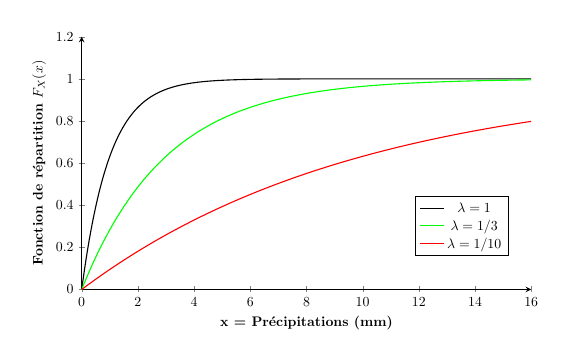
\begin{tikzpicture}[scale = 0.5]
\begin{axis}[
  width=13cm,
  height=8cm,
  xlabel={\textbf{x = Précipitations (mm)}},
  ylabel={\textbf{Fonction de répartition $F_X(x)$}},
  xmin=0, xmax=16,
  ymin=0, ymax=1.2,
  legend style={at={(0.95,0.25)}, anchor=east},
  domain=0:16,
  samples=300,
  axis lines=left,
  thick
]

% λ = 1
\addplot[black, thick] {1 - exp(-1 * x)};
\addlegendentry{$\lambda = 1$}

% λ = 1/3
\addplot[green, thick] {1 - exp(-1/3 * x)};
\addlegendentry{$\lambda = 1/3$}

% λ = 1/10
\addplot[red, thick] {1 - exp(-1/10 * x)};
\addlegendentry{$\lambda = 1/10$}

\end{axis}
\end{tikzpicture}

\end{frame}
\begin{frame}[t]{Exemple 3 (suite)}

Supposons que $\lambda=1/10$. Calculez les quantités suivantes.

\begin{itemize}\itemsep=5mm
\item $P(X\leq 15)$
\item $P(X> 10)$
\item $P(5<X\leq 10)$
\end{itemize}

\vspace{5mm}
\end{frame}

\begin{frame}[t]{Propriétés d'une fonction de répartition}

{\small
\begin{itemize}
 \item[1.] $0\le F_X(x)\le 1$ pour tout $x\in\mathbb{R}$
 \item[2.] $\lim\limits_{x\to\alert{-\infty}}F_X(x)=0$ et $\lim\limits_{x\to\alert{\infty}}F_X(x)=1$
 \item[3.] $F_X$ est \alert{non décroissante} (si $x_1\le x_2$, alors $F_X(x_1)\le F_X(x_2)$)
\end{itemize}

\uncover<2->{
 \begin{itemize}
  \item Pour vérifier si une fonction est une fonction de répartition, on vérifie si elle remplit les 3 propriétés ci-dessus.
  \item De la définition d'une fonction de répartition, on a que  pour tout $a<b$, $P(a<X\le b)=F_X(b)-F_X(a)$.
 \end{itemize}
}
}
\end{frame}

\begin{frame}[t]{}

\begin{Boite}{Variables aléatoires discrètes et continues}
\begin{itemize}\itemsep3mm
\item  Si $F_X$ est une fonction en escalier continue à droite,  alors on dit que $X$ est une variable aléatoire \alert{discrète}.
\item Si $F_X$ est une fonction continue, alors on dit que  $X$ est une variable aléatoire \alert{continue}.
 \end{itemize}
\end{Boite}

 \vspace{3mm}
 Dans ce cours, nous allons nous concentrer sur les variables
 aléatoires \alert{continues}.
\end{frame}

%\section{Variables aléatoires discrètes}
%
%\begin{frame}[t]{Variable aléatoire discrète}
%Les v.a. discrètes sont des v.a. pour lesquelles l'ensemble
%des valeurs possibles est \alert{dénombrable}.
%
%\medskip
%Autrement dit, si $X$ est une v.a. discrète, alors
%son image est de la forme\\
%$R_X=\{x_1,x_2,\ldots,x_m\}$\\
%ou\\
%$R_X=\{x_1,x_2,\ldots\}$.
%\end{frame}
%
%\begin{frame}[t]{Exemples}
%\begin{itemize}
% \item<1-> Considérons le viaduc de l'autoroute Charest surplombant
% l'autoroute Robert-Bourassa. Soit $X$, le nombre de véhicules empruntant
% ce viaduc dans un intervalle de temps donné. Alors $R_X=\{0,1,2,\ldots\}$
% et $X$ est une v.a. discrète.
% \item<2-> On lance un missile dans un champ de tir. Soit $Y$ la v.a. qui vaut
% 1 si le missile tombe à moins de 10 m de sa cible et qui vaut 0 sinon. Alors
% $R_Y=\{0,1\}$ et $Y$ est une v.a. discrète.
%\end{itemize}
%\end{frame}
%
%\begin{frame}[t]{Fonction de probabilité/masse}
%On a déjà vu que le comportement aléatoire de \alert{toute}
%v.a. $X$ peut être complètement spécifié par sa
%fonction de répartition. Si $X$ est une v.a. discrète, alors
%une autre fonction permet aussi de complètement spécifier
%sont comportement aléatoire.
%
%\uncover<2->{
% \begin{Boite}{Définition}
%  Soit $X$ une v.a. \alert{discrète} et considérons la fonction
%  $p_X:\mathbb{R}\to[0,1]$ qui associe la valeur $p_X(x)=P(X=x)$
%  à tout $x\in R_X=\{x_1,x_2,\ldots\}$. On appelle $p_X$
%  \alert{fonction de probabilité} (ou \alert{fonction de masse},
%  ou \alert{fonction de masse de probabilité}) de $X$.
% \end{Boite}
%}
%
%\uncover<3->{
%Dans l'exemple du dé balancé, la fonction de probabilité
%de $Y$ est $p_Y(-1)=3/6$, $p_Y(1)=3/6$.
%}
%\end{frame}
%
%\begin{frame}[t]{Propriétés de la fonction de probabilité}
%\begin{itemize}
% \item<1->[1.] $p_X(x_i)\ge0$, $i=1,2,\ldots$
% \item<2->[2.] $\sum\limits_{i:x_i\in R_X} p_X(x_i)=1$
%\end{itemize}
%
%\uncover<3->{
%  Pour voir si une fonction est une fonction de probabilité,
%  il suffit de vérifier si elle possède les deux propriétés ci-dessus.
%}
%\end{frame}
%
%\begin{frame}[t]{Lien entre fonctions de probabilité et de répartition}
%\begin{itemize}
%  \item<1-> Si on connait la fonction de répartition, on peut en déduire la fonction
%  de probabilité car
%  \begin{align*}
%  p_X(x_i)&=P(X=x_i)=P(x_{i-1}<X\le x_i)\\
%  &=F_X(x_i)-F_X(x_{i-1}).
%  \end{align*}
%  \item<2-> Si on connait la fonction de probabilité, on peut en déduire la fonction
%  de répartition car
%  \begin{align*}
%  F_X(x_i)&=P(X\le x_i)=P(X=x_1\text{\ ou\ }X=x_2\text{\ ou\ }
%  \cdots\text{\ ou\ }X=x_i)\\
%  &=\sum_{j=1}^ip_X(x_j).
%  \end{align*}
%\end{itemize}
%\end{frame}
%
%\begin{frame}[t]{Exemple}
%Supposons que nous tirons de fa\c{c}on indépendante 4 boules
%\alert{avec remise} d'une urne qui contient 7 boules bleues
%et 3 boules rouges. Soit $X$, le nombre de boules rouges
%obtenues. Quelle est la fonction de probabilité de $X$?
%(Décrivez la de fa\c{c}on mathématique, à l'aide
%d'un tableau et à l'aide d'un diagramme.) Faites
%un graphe de la fonction de répartition de $X$.
%
%\medskip
%{\bf \underline{Mathématiquement}:}
%\end{frame}
%
%\begin{frame}[t]{Exemple (suite)}
%
%{\bf \underline{Tableau}:}
%
%\vspace{1in}
%
%{\bf \underline{Diagramme}:}
%\end{frame}
%
%\begin{frame}[t]{Exemple (suite)}
%
%{\bf \underline{Fonction de répartition}:}
%\end{frame}
%
\section{Fonction de densité $f_X$}


\begin{frame}[t]{V. a. continues: fonction de densité $f_X$}

{\small
Pour une v.a. $X$ continue, $F_X$ est continue
pour tout $x\in\mathbb{R}$. }
\begin{Boite}{Fonction de densité $f_X$}


La fonction $\displaystyle f_X(x)=\frac{d}{dx}F_X(x)$ est appelée \alert{fonction de densité
de probabilité} (ou \alert{fonction de densité}) de $X$.
\end{Boite}

\begin{Boite}{Lien entre répartition $F_X$ et densité $f_X$}
\begin{align*}
 F_X(x)&=\int_{-\infty}^x f_X(u)\;du \\
 P(a<X\le b)&=F_X(b)-F_X(a)=\int_a^bf(u)\;du.
\end{align*}
\end{Boite}

\end{frame}

\begin{frame}[t]{Probabilité = aire sous la densité}
\begin{center}
    
\begin{tikzpicture}[scale=0.9]

% Axes
\draw[->, thick] (-1.2,0) -- (5.5,0) node[right] {$x$};
\draw[->, thick] (0,-0.1) -- (0,2.2) node[above left] {$f_X(x)$};

% Courbe rouge (densité stylisée)

\draw[red, thick] (-0.8,0) -- (0.5,0);  % Avant densité
\draw[red, thick] (0.5,0) -- (2,1.5);  % Avant densité
\draw[red, thick] (2,1.5) -- (3,1.5);  % Avant densité
\draw[red, thick] (3,1.5) -- (4.5,0);  % Avant densité

\draw[red, thick] (4.5,0) -- (5.2,0);   % Après densité

% Hachures entre a et b
\begin{scope}
  \clip (2,0) rectangle (3,1.5);
  \foreach \x in {2.05,2.15,...,2.95}
    \draw[pattern=north east lines, pattern color=black!70] (\x,0) -- (\x,1.5);
\end{scope}

% Traits verticaux pour a et b
\draw[dashed] (2,0) -- (2,1.5);
\draw[dashed] (3,0) -- (3,1.5);

% Labels a, b
\node at (2,-0.2) {$a$};
\node at (3,-0.2) {$b$};

% Domaine Rx
\draw[<->] (0.5,-0.6) -- (4.5,-0.6) node[midway, below] {$\mathbb{R}_X$};

\end{tikzpicture}
\end{center}

{\small
$f_X$ n'est \alert{pas} une probabilité (elle peut prendre des valeurs
supérieures à 1), mais son intégrale sur une région donne la
probabilité que $X$ prenne une valeur dans cette région. % Comme $f(x)\Delta x\approx F(x+\Delta x)-F(x)$ quand $\Delta x$ est petit, la densité est proportionnelle à la probabilité que $X$ prenne une valeur dans le petit intervalle $(x,x+\Delta x)$.
}
\end{frame}

\begin{frame}[t]{Propriétés d'une fonction de densité}

\begin{itemize}
 \item[1.] $f_X(x)\ge0$ pour tout $x\in\mathbb{R}$
 \item[2.] $\displaystyle\int_{-\infty}^\infty f_X(x)\;dx=1$
 \item[3.] $f_X$ est continue par morceaux
 \item[4.] si $x\notin \mathbb{R}_X$, alors $f_X(x)=0$ %(et donc  $\int_{-\infty}^\infty f(x)\;dx=1$)
\end{itemize}

\uncover<2->{
Comme $\displaystyle\int_a^af(u)\;du=0$,
alors $P(X=a)=0$ pour tout $a\in\mathbb{R}$ dans le cas
d'une v.a. \underline{continue}. Ceci implique que
$$
\left.\begin{array}{l}
P(a<X<b)\\P(a<X\le b)\\P(a\le X<b)\\P(a\le X\le b)
\end{array}\right\}=\int_a^bf_X(u)\;du.$$}

\end{frame}


\begin{frame}[t]{Exemple 4}

{\small
Soit une v.a. $X$ continue pouvant prendre toute valeur dans l'intervalle
$[0,20]$. On vous dit que
\begin{itemize}
\item tous les intervalles de même longueur dans $[0,10)$ sont équiprobables,
\item tous les intervalles de même longueur dans $[10,20]$ sont équiprobables,
\item un intervalle dans $[10,20]$ est deux fois plus probable qu'un intervalle de même longueur dans $[0,10)$.
    \end{itemize}
Déterminez la densité de $X$, sa fonction de répartition, et évaluez $P(5<X<12)$.}
\end{frame}

\begin{frame}[t]{Exemple 4(suite)}
\end{frame}

\begin{frame}[t]{Exemple 5: Retour à l'exemple de la pluie}
La distribution de la quantité de pluie mensuelle re\c{c}ue à la station
est définie par $F_X(x)=1-e^{-\lambda x}$ si
$x\ge0$, et $0$ ailleurs.
\begin{itemize}\itemsep 2cm
\item Quelle est la densité de $X$?
\item Quelle est la probabilité que la quantité de pluie re\c{c}ue excède 5 mm?
%\item Quelle est la probabilité de recevoir entre 10 et 15 mm sachant que l'on recevra au moins 5 mm?
\end{itemize}
\end{frame}

\begin{frame}[t]{Exemple 5 (suite)}
\begin{itemize}
\item Quelle est la probabilité de recevoir entre 10 et 15 mm sachant que l'on recevra au moins 5 mm?
\end{itemize}

\end{frame}

\begin{frame}{Remarque}
    La notation «rigoureuse» est $F_X$ et $f_X$ pour les fonctions de répartition et de densité de la variable aléatoire $X$. Par contre, pour simplifier l'écriture, lorsqu'il est question d'une seule variable aléatoire, on omet l'indice et on écrit $F$ et $f$.
\end{frame}

\section[Espérance-Variance]{Espérance et variance d'une variable aléatoire}

\subsection*{ }

\begin{frame}[t]{Aspects importants d'une distribution}
$F$ ou $f$ spécifie complètement la distribution de la variable aléatoire $X$.

\medskip
%Dans bien des cas, %on n'a pas besoin de conna\^{\i}tre la distribution de $X$ en entier, mais seulement quelques-unes de ses
Il est utile de s'intéresser aux caractéristiques qui résument les aspects
principaux de son comportement.

\medskip
\begin{itemize}\itemsep2mm
\item tendance centrale
\item dispersion
\item forme
\end{itemize}

\end{frame}

\begin{frame}[t]{Mesure de la tendance centrale}%: la moyenne théorique (espérance de X)}
%La \alert{moyenne théorique} d'une v.a. $X$, aussi appelée l'\alert{espérance} de $X$, fournit une indication sur la tendance centrale (i.e., le milieu) d'une distribution.

\begin{Boite}{Espérance de $X$}
 L'\alert{espérance} (moyenne théorique) d'une v.a. $X$ est donnée par
 $$
 E(X)=\mu=\int_{-\infty}^\infty xf(x)\;dx.$$
C'est la valeur moyenne que l'on obtiendrait si on réalisait l'expérience aléatoire une infinité de fois (donc si on obtenait une infinité de valeurs de $X$ réparties selon $F$).
\end{Boite}

\end{frame}

%\begin{frame}[t]{Exemple avec une v.a. discrète}
%
%{
% \small Une étude permet de croire que la mise en marché du
% produit X-12 rapportera un profit selon la distribution suivante:
% \begin{center}
%  \begin{tabular}{c|cccccc}
%  Profit & -10\$ & -1\$ & 0\$ & 1\$ & 2\$ & 5\$ \\ \hline
%  Probabilité & 0.1 & 0.2 & 0.1 & 0.1 &  0.2 & 0.3
%  \end{tabular}
% \end{center}
%
%\smallskip
%Quel est la moyenne de la distribution du profit (ou
%la valeur moyenne du profit, ou le profit moyen, ou le profit espéré)?
%}
%\end{frame}

\begin{frame}[t]{Exemple 6: Retour à l'exemple de la pluie}

 {\small $f(x)=\left\{\begin{array}{c l}\lambda e^{-\lambda x}&\text{si} \;x>0\\
 0&\text{si} \; x\leq 0
 \end{array}\right.$

\vspace{3mm}

Quelle quantité de pluie tombe-t-il en moyenne durant ce mois? (Répondez pour $\lambda$ en général, sans fixer de valeur).
}



 %\vspace{-3cm}
 %Quelle quantité de pluie tombe-t-il en moyenne durant ce mois? (Répondez pour $\lambda$ en général, sans fixer de valeur).

\end{frame}




% \begin{frame}[t]{Variabilité d'une variable aléatoire (variance de X)}

% {\small Deux variables aléatoires peuvent avoir la \underline{même moyenne},
%  mais l'une peut être beaucoup \underline{plus variable
%  que l'autre}, i.e., à avoir tendance à prendre des valeurs
%  plus éloignées de sa moyenne que l'autre.

%  \medskip
%  {\bf \underline{Expérience}:} Rouler 30 dés réguliers.

%  $X_1=$ la valeur indiquée par le premier dé\\
%  $X_2=$ la somme des valeurs indiquées par les 30 dés, divisée par 30.

%  \medskip
%  On peut montrer que $X_1$ et $X_2$ ont la même
%  moyenne ($3,5$).

%  \medskip
%  Cependant, $X_2$ aura tendance à prendre
%  des valeurs très proches de $3,5$, alors que $X_1$ peut prendre
%  n'importe quelle valeur entre 1 et 6 avec la même probabilité.
% }
% \end{frame}

\begin{frame}[t]{Variabilité d'une variable aléatoire}

{\small    Deux variables aléatoires peuvent avoir la \underline{même espérance}, mais l'une peut être \underline{plus variable que l'autre}, i.e., à avoir tendance à prendre des valeurs plus éloignées de sa moyenne que l'autre.

 \medskip
 {\bf \underline{Exemple}:} Nous avons deux sacs. Dans le premier, il y a dix boules numérotées de 1 à 10 et dans le deuxième, il y a deux boules numérotées 5 et 6.

 L'expérience consiste à piger une boule dans chaque sac.

 $X=$ la valeur indiquée par la boule du premier sac\\
 $Y=$ la valeur indiquée par la boule du deuxième sac.

 \medskip
 On peut montrer que $X$ et $Y$ ont la même espérance ($5,5$).

 \medskip
 Cependant, on voit très bien que les résultats de $X$ seront plus variables.
 }
\end{frame}

\begin{frame}[fragile]
\frametitle{Variabilité d'une variable aléatoire}
{\small
Voici 10 réalisations de l'expérience:

\begin{verbatim}
      X     Y
 [1,] 4     6
 [2,] 9     5
 [3,] 6     5
 [4,] 3     6
 [5,] 5     5
 [6,] 9     6
 [7,] 1     6
 [8,] 6     5
 [9,] 7     6
[10,] 2     5
\end{verbatim}
}
\end{frame}

\begin{comment}
    \begin{frame}[t]{Fonctions de probabilité de $X_1$ et $X_2$}

{\small La figure ci-dessous montre la fonction de probabilité de $X_1$
en bleu et celle de $X_2$ en rouge. Même si les deux v.a. ont la même
moyenne, on voit bien que la distribution de $X_2$ est beaucoup
plus concentrée autour de 3,5 que celle de $X_1$.

\centerline{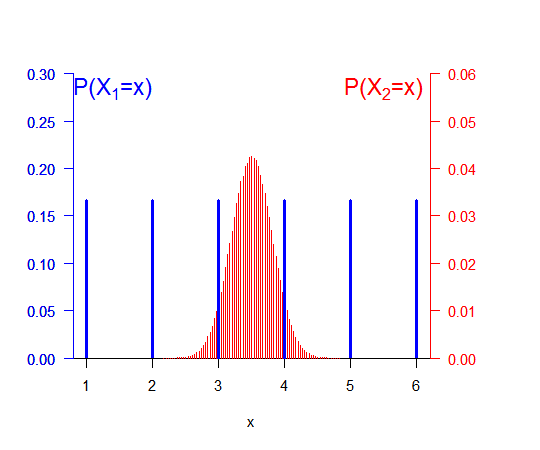
\includegraphics[height=2.1in]{Images/Module 2/pmf-x1x2-modif.png}}

%(Note: Pour $P(X_2=x)$, les barres rouges ne sont pas à l'échelle et n'apparaissent pas pour toutes les valeurs de $R_{X_2}$.)
}
\end{frame}
\end{comment}


\begin{frame}[t]{Mesure de dispersion d'une distribution}

\begin{Boite}{Variance et écart-type}
 \begin{itemize}
  \item La \alert{variance} d'une variable $X$ (ou de la distribution de $X$)
  est donnée par
  $$V(X)=\sigma^2=\int_{-\infty}^\infty (x-\mu)^2f(x)\;dx.$$
  \item L'\alert{écart-type} de $X$ est $\sigma=\sqrt{\sigma^2}$.
 \end{itemize}
\end{Boite}
\end{frame}

\begin{frame}[t]{Exemple 7: Retour à l'exemple de la pluie}

La quantité de pluie reçue en un mois à cette station est-elle très variable?
\end{frame}

\section[Fonction de $X$]{Espérance d'une fonction de variable aléatoire }

\subsection*{ }

\begin{frame}[t]{Valeur espérée d'une fonction de $X$}

{\small
\begin{Boite}{Espérance d'une fonction de $X$}
 Soit $X$ une v.a. et posons $Y=H(X)$ une fonction
 de $X$. Alors l'\alert{espérance mathématique
 de $H(X)$} (ou de $Y$) est définie par
 $$E[Y]=E[H(X)]=\int_{-\infty}^\infty H(x)f(x)\;dx.$$
\end{Boite}
Un cas particulier...
\begin{itemize}
% \item<2-> $H(X)=X\Rightarrow E[X]=\mu$, donc la valeur espérée de $X$, ou l'espérance de $X$, ou la moyenne de $X$ sont toutes des expressions équivalentes  pour $\mu$.
 \item $H(X)=(X-\mu)^2\Rightarrow E[(X-\mu)^2]=V[X]=\sigma^2=\;\;$variance de $X$.
\end{itemize}
}
\end{frame}

\begin{frame}[t]{Résultats utiles}

Supposons que $a$ et $b$ sont des constantes.

\begin{itemize}
\item<1-> $E[aX+b]=aE[X]+b$\ \ \ \ \
%\underline{Preuve}:

\vspace{0.45in}

\item<1-> $V[X]=E[X^2]-(E[X])^2$\ \ \ \ \
%\underline{Preuve}:

\vspace{0.75in}

\item<1-> $V[aX+b]=a^2V[X]$\ \ \ \ \
%\underline{Preuve}:
\end{itemize}
\end{frame}

\begin{frame}[t]{Exemple 8: Retour à l'exemple de la pluie}

Supposons que les revenus (en centaines de milliers de dollars)
générés par un barrage sont bien modélisés par l'équation $R=10+3X$ (où $X$ est la quantité de pluie). Quelle est la valeur
moyenne et l'écart-type de ces revenus?

Rappel: $E(X)=1/\lambda\qquad V(X)=1/\lambda^2$
\end{frame}




\begin{frame}[t]{Réponses aux exemples}

\scriptsize
\begin{enumerate}
  \item (pas de question)
  \item $P(Y=-75)=1/2$, $F(y)=\left\{
      \begin{array}{ll}
      0 & \text{ si } y<-75\\
      1/2 & \text{ si } -75\leq y<50\\
      1 & \text{ si } y\geq 50\\
      \end{array}\right.$
  \item $P(X\leq 15)\approx0,777,\quad P(X> 10)\approx 0,368, \quad P(5<X\leq 10)\approx 0,239$
  \item $f(x)=\left\{
      \begin{array}{ll}
      1/30 & \text{ si } 0\leq x <10\\
      2/30 & \text{ si } 10\leq x\leq20\\
      0 & \text{ sinon }\\
      \end{array}\right.$, $F(x)=\left\{
      \begin{array}{ll}
      0 & \text{ si } x<0\\
      x/30 & \text{ si } 0\leq x <10\\
      (2x-10)/30 & \text{ si }  10\leq x \leq20\\
      1 & \text{ si } x>20\\
      \end{array}\right.$
      $P(5<X<12)=F(12)-F(5)=\displaystyle\int_5^{10}\frac{1}{30}dx+\int_{10}^{12}\frac{2}{30}dx=$aire des  rectangles
  \item $f(x)=\left\{
      \begin{array}{ll}
      \lambda e^{-\lambda x} & \text{si }  x \geq 0\\
      0 & \text{sinon }\\
      \end{array}\right.,\; P(X>5)=e^{-5\lambda},\; P(10\leq X\leq 15|X\geq5)=\frac{e^{-10\lambda}-e^{-15\lambda}}{e^{-5\lambda}}$
  \item $E(X)=1/\lambda$
  \item $V(X)=1/\lambda^2$
  \item $E(R)=10+3/\lambda,\quad \sigma=3/\lambda$
 \end{enumerate}
\end{frame}



\end{document}